\chapter{OUTPUT AND ANALYSIS}
This is what our UI of our web application looks like on 'OFF' (\ref{fig:dashboardoff}) and 'ON' (\ref{fig:dashboardon}):
\begin{figure}[h]
    \centering
    \begin{minipage}{1\textwidth}
        \centering
    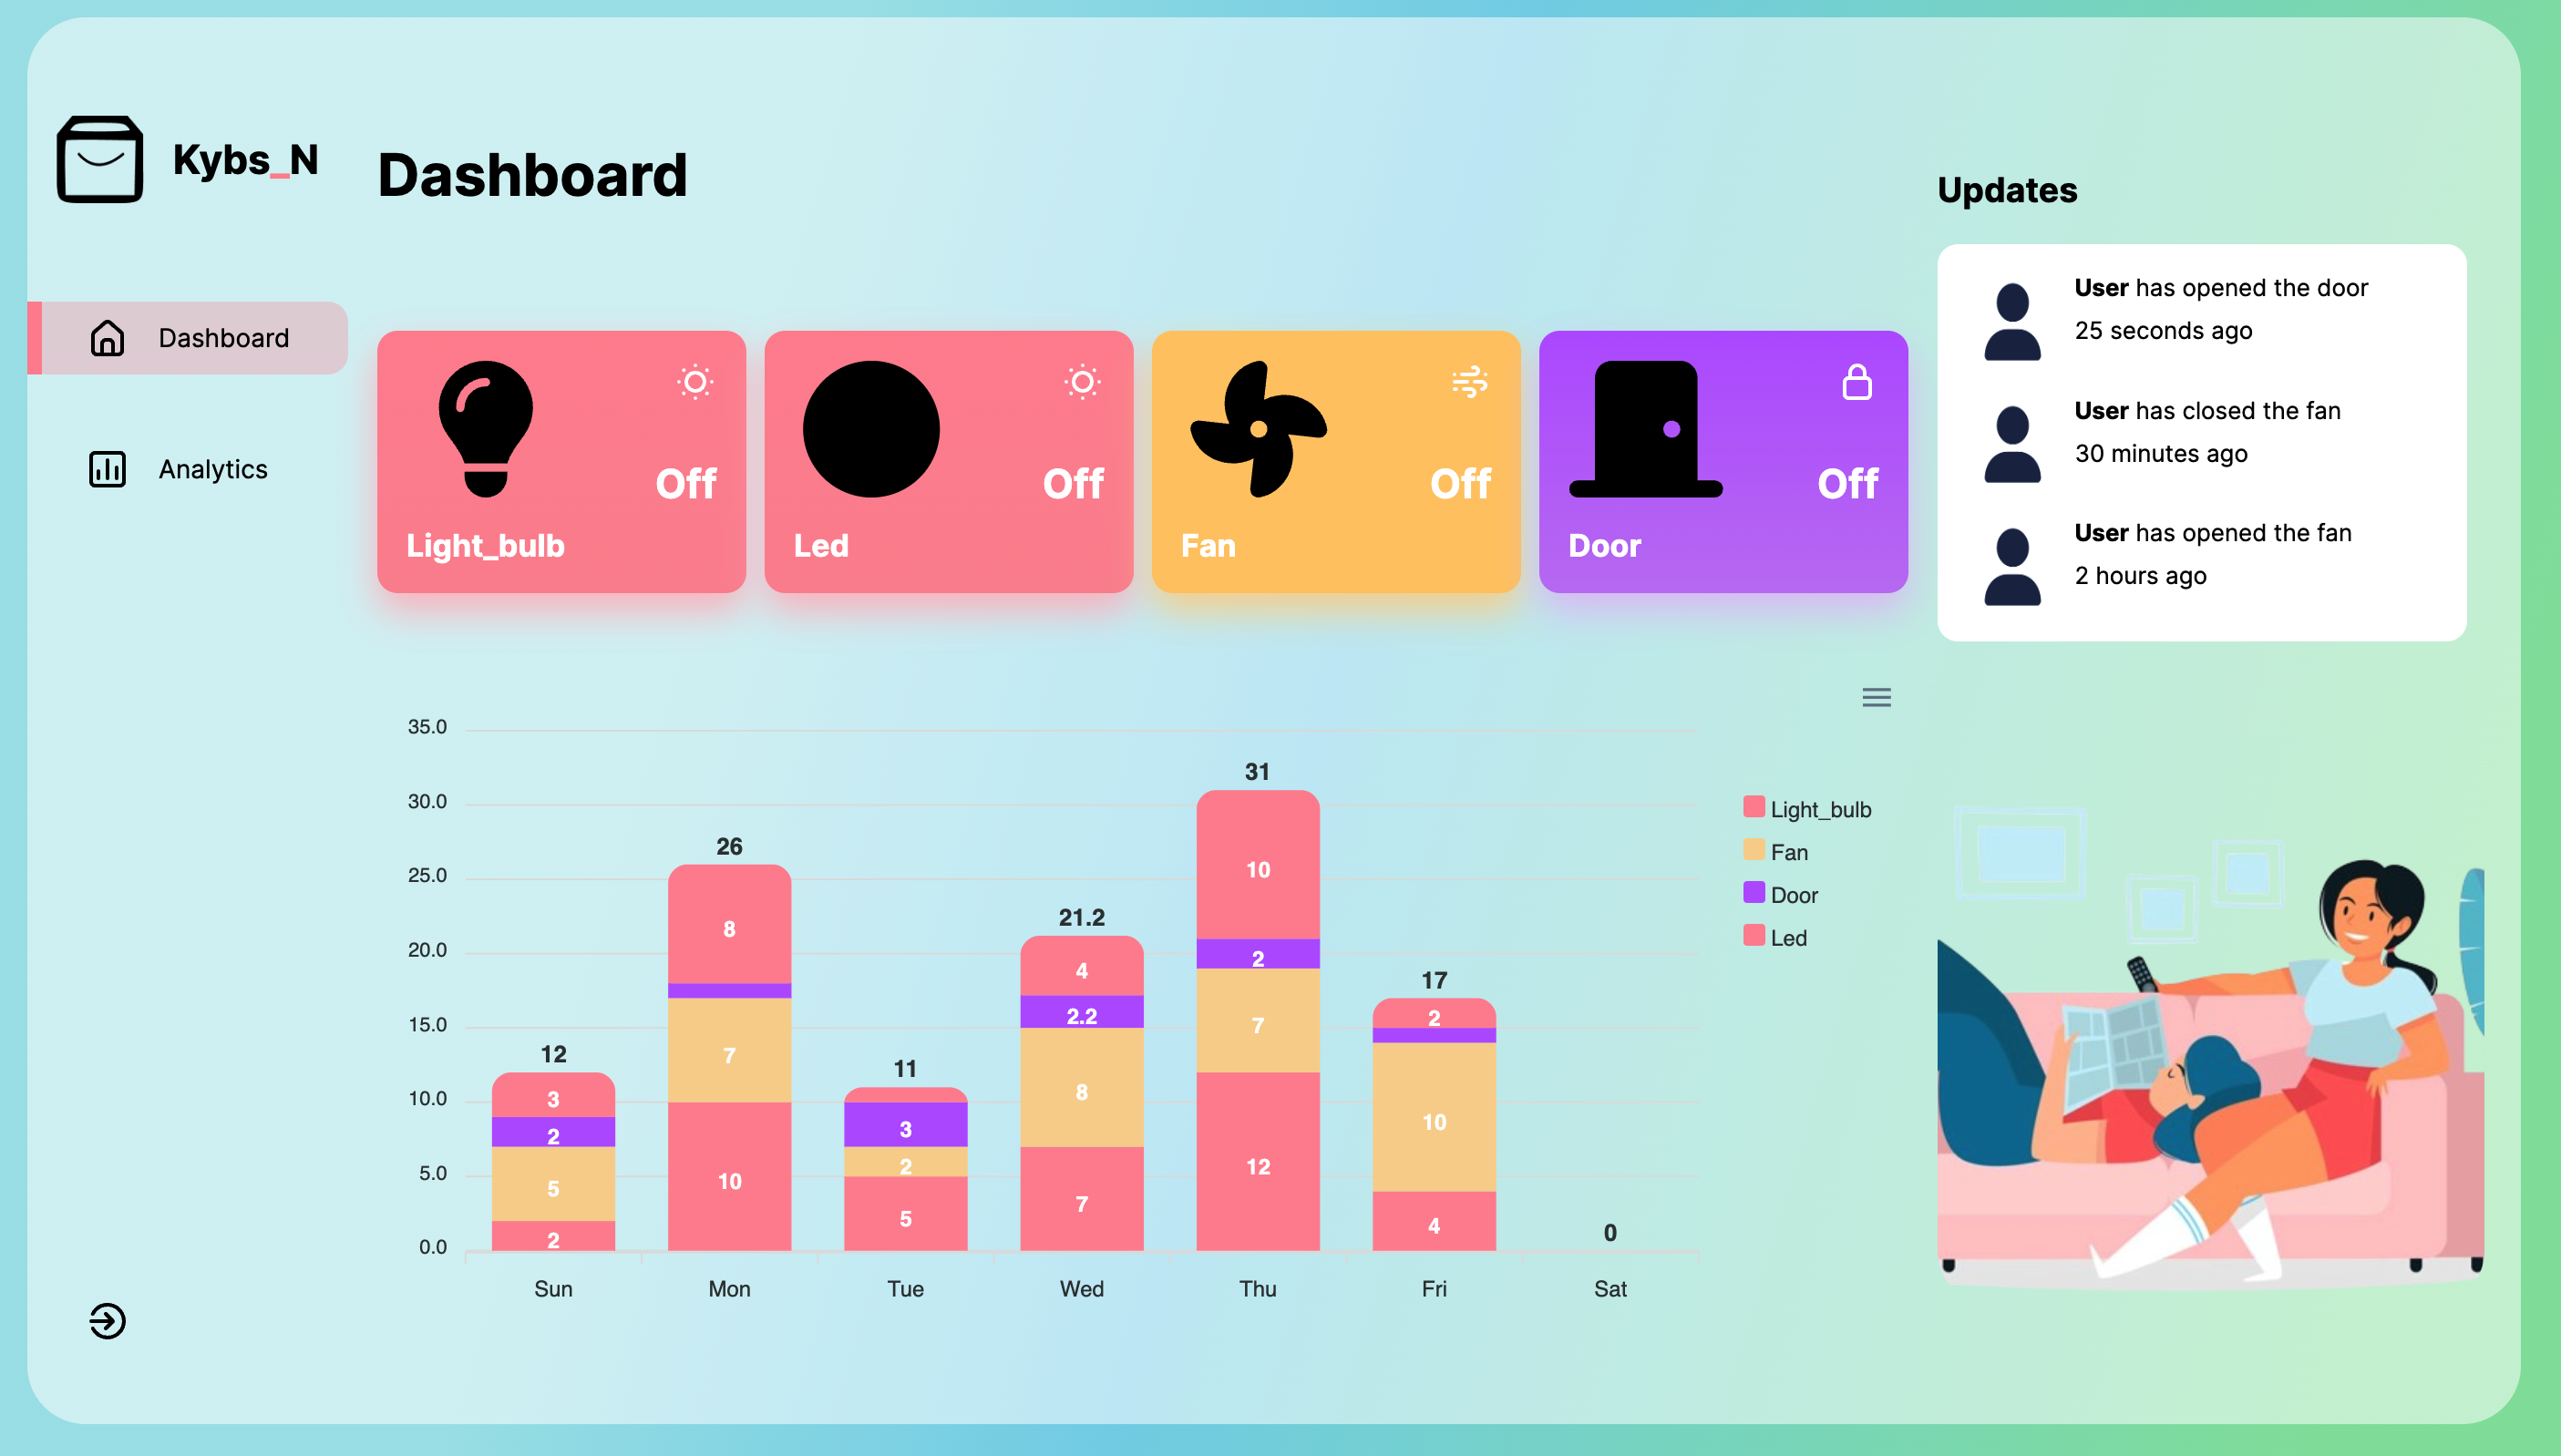
\includegraphics[width=1\textwidth]{dashboardOff}
    \caption{Web Application UI when devices are “OFF”}
    \label{fig:dashboardoff}
    \end{minipage}
    \begin{minipage}{1\textwidth}
        \centering
    \includegraphics[width=1\textwidth]{dashboardOn}
    \caption{Web Application UI when devices are “ON”}
    \label{fig:dashboardon}
    \end{minipage}
\end{figure}

The above figures show the UI of our web application we have made in React, when they are “On” and “Off”. In the landing page of this web page we can see 3 different sections. 
Left section shows different options of Dashboard and Analytics. Currently there is nothing in the Analytics section.\\
The main part of this dashboard is in the middle section which shows the status of all the appliances which are controlled by our automation system. It shows if the device is “On” or “Off”, on clicking the device card we can see the analytics. It shows the data of the device on how long (in hour) they were in “On” state. An area plot is given for better visualization of the data. Below it is a bar graph showing the cumulative data of all individual devices.\\
Right section shows the recent commands given to devices and how long has it been since the command was given.\\

The complete system is shown in \ref{fig:home}.
\begin{figure}[h]
    \centering
    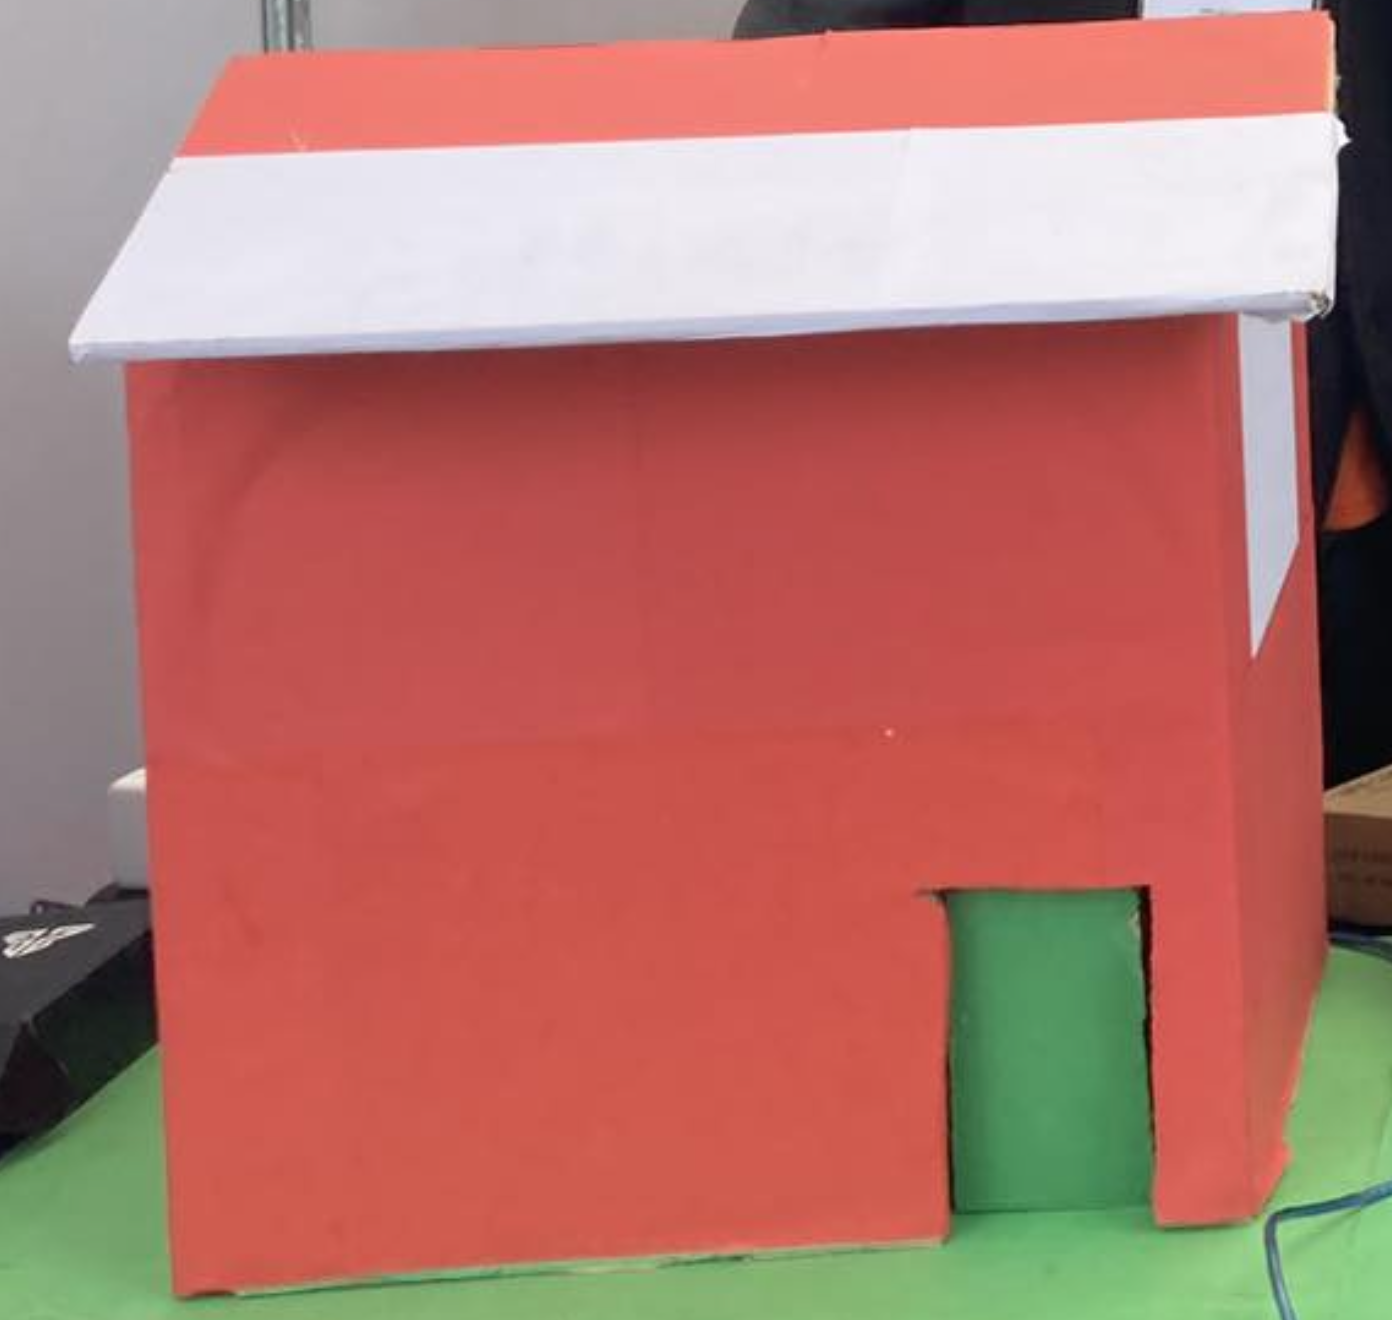
\includegraphics[width = 0.8\textwidth]{home}
    \caption{House}
    \label{fig:home}
\end{figure}
